\chapter{Contexto y estado de la técnica}

\section{Introducción a la computación cuántica}

En la segunda mitad del siglo XX, en plena revolución científica de la física de partículas, la física teórica entre otras ramas, se inició un nuevo campo del conocimiento, la computación cuántica. Esta nueva rama del conocimiento es descendiente directa de dos de las teorías físicas mas importantes que vieron su nacimiento en la primera mitad del siglo XX. Por un lado, la mecánica cuántica, teoría que da cuenta del comportamiento de la materia a pequeña escala, la cual fue desarrollada principalmente desde finales del siglo XIX hasta los años 40 del siglo XX. Por otro lado, la teoría de la información fundada por Shannon en su famoso artículo de 1948 \textit{A Mathematical Theory of Communication} \citep{Shannon1948}. En ese trabajo se introduce la teoría matemática detrás del concepto de información, estableciendo ideas clave como la entropía de la información, entre otras. Shannon propuso un marco teórico que revolucionó nuestra comprensión de cómo la información es una magnitud física medible. \\

En un artículo de 1980, Paul Benioff introduce la idea de una computadora modelada como un sistema físico cuántico \citep{benioff}, abriendo nuevas posibilidades en la intersección entre la computación y la física fundamental. Posteriormente al artículo de Benioff, en una conferencia de 1982 \citep{richard}, Richard Feynman apoyado en el artículo de Benioff planteó la idea de utilizar sistemas basados en las reglas de la mecánica cuántica para simular sistemas cuánticos y poder superar así las limitaciones presentes en el paradigma de computación clásico. En esta época se conocían ya las limitaciones de computo existentes para simular sistemas cuánticos grandes como moléculas. \\

Desde entonces, se ha explorado la posibilidad de utilizar el marco teórico de la mecánica cuántica para poder diseñar algoritmos que superen a sus contrapartes clásicos. Este hecho no se vio confirmado hasta que en 1992, se publico un trabajo, en el cual sus autores plateaban, por primera vez, un algoritmo cuántico capaz de resolver una tarea especifica, con una complejidad de resolución menor que cualquier posible algoritmo clásico existente \citep{deutsch}. El problema a resolver consistía en clasificar si una función discreta dada era constante o balanceada. \\

Posteriormente, numerosos algoritmos cuánticos han surgido, confirmando la hipótesis planteada por Feynman y Benioff de la utilidad de la mecánica cuántica como marco para el diseño de algoritmos cuánticos. Uno de los algoritmos más famosos e importantes del campo, es el propuesto por Peter Shor de 1994 \citep{shor}, el cual permite encontrar los factores primos de cualquier número de forma eficiente. \\

La computación cuántica es un nuevo paradigma de procesamiento de la información que se basa en el marco de la mecánica cuántica para implementar nuevas operaciones no presentes en el formalismo clásico de computación. La unidad de información fundamental con la que se opera en este nuevo marco de computación no es el bit, el cual es un escalar, si no que es un nuevo objeto, el qubit. Dado que la computación cuántica se basa en la aplicación de las reglas de la mecánica cuántica, el formalismo de la computación cuántica es en esencia el formalismo de la mecánica cuántica. Bajo este marco teórico, la unidad de información básica, el qubit, representa un sistema cuántico de dos niveles, dos estados, bien diferenciados. Estos estados representan dos vectores del espacio vectorial usado para describir el sistema. En una notación compacta, denominada notación de Dirac \citep{dirac1939}, los dos estados cuánticos base del qubit representados por vectores vienen dados por la ecuación  \ref{eq: estados_qubits}.  


\begin{equation}
    \ket{0} = 
    \begin{pmatrix}
        1 \\
        0
    \end{pmatrix}
    ;
    \quad
    \ket{1} = 
    \begin{pmatrix}
        0 \\
        1
    \end{pmatrix}
    \label{eq: estados_qubits}
\end{equation}


Estos estados base, son vectores del espacio de Hilbert, $\mathcal{H}$. El hecho de que el formalismo necesario para describir el estado de un qubit sea el de un espacio vectorial produce que, a diferencia de los bits clásicos, el estado en el que se encuentra un qubit puede no ser ya solo $0$ o $1$, si no que puede ser cualquier combinación linear de los vectores base $\ket{0}$ y $\ket{1}$. Dado que además, los vectores son base del espacio de Hilbert, esta combinación linear puede contener coeficientes complejos. Es decir, dado un qubit, este puede encontrarse en el estado $\ket{\psi}$, que viene dado por la ecuación \ref{eq:estado_psi}.

\begin{equation}
    \ket{\psi} = \alpha\ket{0} + \beta\ket{1} \; \; \; \; \; \alpha, \beta \in \mathbb{C}
    \label{eq:estado_psi}
\end{equation}

La relación dada por \ref{eq:estado_psi} permite generar infinitos estados $\ket{\psi}$ dado los estados base $\ket{0}$ y $\ket{1}$.

\newpage

El espacio de Hilbert \citep{casazza} de un qubit es un espacio vectorial complejo de dimensión 2, $\mathbb{C}^{2}$. Los vectores unitarios de este espacio complejo de dimensión 2 pueden visualizarse mediante la denominada esfera de Bloch \citep{bloch}. La esfera de Bloch es la representación geométrica del espacio de Hilbert de un qubit. Esta representación permite entender de forma sencilla e intuitiva los estados cuánticos en los que se puede encontrar un qubit. La Figura \ref{fig:bloch_sphere} muestra la visualización de la esfera de Bloch.


\begin{figure}[!ht]
    \centering
    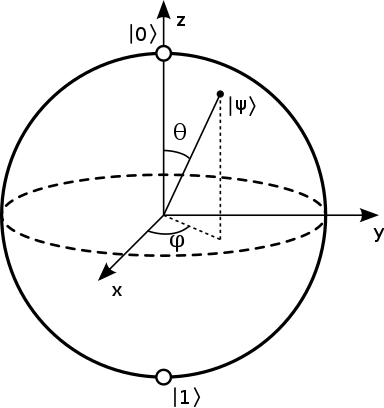
\includegraphics[scale = 0.5]{img/03-esfera_bloch.png}
    \caption{esfera de Bloch para un qubit.}
    Fuente: adaptada de \cite{bloch}
    \label{fig:bloch_sphere}
\end{figure}

Cada punto de la superficie de la esfera representa cada uno de los estados cuánticos puros, en los que se puede encontrar un qubit. Entendiendo como estado cuántico puro el estado que representa completamente la información sobre el sistema en cuestión, es decir, proporciona una descripción completa y detallada de las propiedades cuánticas del sistema. Bajo el marco de la esfera de Bloch, los coeficientes de la ecuación \ref{eq:estado_psi} pueden escribirse en función de los ángulos internos que fijan el estado $\ket{\psi}$, reescribiendo la ecuación por la expresión dada por la ecuación \ref{eq:estado_bloch}.


\begin{equation}
    \ket{\psi} = \cos{\frac{\theta}{2}}\ket{0} + e^{i\phi}\sin{\frac{\theta}{2}}\ket{1}
    \label{eq:estado_bloch}
\end{equation}

La utilidad de la esfera de Bloch queda limitada a solo un qubit, ya que si se quiere describir el estado conjunto $\ket{\psi'}$ que representa el estado global de dos qubits o más, la esfera de Bloch no es útil, dado que el espacio de Hilbert del estado $\ket{\psi'}$ es de dimensión mayor de 2. 

\newpage

El espacio de Hilbert conjunto del $\ket{\psi'}$ que describe el estado de $n$ qubits no es mas el producto tensorial de los espacios individuales de cada qubit. Sea $\mathcal{H}$ el espacio de Hilbert de un qubit, el espacio de Hilbert de $n$ viene dado por $\ket{\psi'} \in \mathcal{H}^{\otimes n}$. Esto hace inviable una representación fidedigna del estado mediante la esfera de Bloch.\\

Realizar operaciones en el paradigma de computación cuántica, consiste en realizar transformaciones a los qubits de tal forma que el vector $\ket{\psi}$ de cada qubit cambie de posición dentro de su esfera de Bloch individual. Sin embargo hay una serie de sutilezas matemáticas que deben exponerse antes de continuar. \\

Dado que trabajamos en el marco de la mecánica cuántica es necesario presentar algunos de los postulados y restricciones matemáticas que se imponen dentro de la propia teoría cuántica \citep{cohen}. En primer lugar, los vectores $\ket{\psi}$ que describen los estados cuánticos de un qubit o conjuntos de qubits, deben ser unitarios. Matemáticamente esta condición viene expresada por la ecuación \ref{eq:unitariedad}. 

\begin{equation}
    |\braket{{\psi}|{\psi}}| = 1
    \label{eq:unitariedad}
\end{equation}

La interpretación física de esta condición implica que los estados cuánticos usados para describir un sistema, es decir, un conjunto de qubits, son completos, contienen toda la información necesaria para describir en su totalidad al sistema. Esta es la razón por la cual, los estados cuánticos puros de un qubit, son aquellos que se encuentran en la superficie de la esfera de Bloch (Figura \ref{fig:bloch_sphere}) ya que son aquellos estados que tienen norma unidad. \\

En segundo lugar, las operaciones que se implementan para operar sobre un estado $\ket{\psi}$ dado deben ser operaciones unitarias. Las operaciones en computación cuántica vienen descritas por operadores, los cuales son objetos matemáticos que realizan transformaciones sobre un estado cuántico dado. Los operadores, deben ser unitarios, esto implica que las transformaciones y operaciones que se realicen sobre un estado $\ket{\psi}$ no deben cambiar la norma del mismo. Matemáticamente la condición de  unitariedad dado un operador $U$ viene dada por la ecuación \ref{eq:operador_unitario}.

\begin{equation}
    U U^{\dagger} = U^{\dagger} U = I
    \label{eq:operador_unitario}
\end{equation}

\newpage

La condición de unitariedad es un restricción que debe cumplir cualquier operación que actúe sobre qubits, con la salvedad de la operación de medida, usada para extraer la información del sistema. En computación cuántica los operadores representan rotaciones dentro de la esfera de Bloch. Los operadores pueden actuar sobre uno o varios qubits de forma simultanea. Dado que estamos operando sobre unidades de información, utilizaremos la palabra puerta cuántica y operador cuántico de forma indistinta durante el presente documento.  \\

Para aliviar el uso de la notación, durante años se ha ido desarrollando notación abstracta la cual permite identificar distintas operaciones que pueden realizarse sobre los qubits \citep{diVincenzo}. Un ejemplo de puerta cuántica es la dada por la expresión \ref{eq:operador_x}.


\begin{equation}
    X = \begin{bmatrix}
    0 & 1 \\
    1 & 0 \\
    \end{bmatrix}
    \label{eq:operador_x}
\end{equation}

La acción de esta puerta, que solo actúa sobre un qubit, cambia o invierte el estado original del qubit. La ecuación \ref{eq:operador_x_estado} da cuenta de la acción de la puerta sobre un qubit en un estado general $\ket{\psi}$.

\begin{equation}
    X \ket{\psi} = X(\alpha\ket{0} + \beta\ket{1}) = \beta\ket{0} + \alpha\ket{1}
    \label{eq:operador_x_estado}
\end{equation}

En términos de la esfera de Bloch, se ha desplazado el estado del qubit desde un punto dado de la superficie de la esfera hasta aquel situado en el punto diametralmente opuesto. El operador que permite realizar un desplazamiento genérico para desplazar el estado $\ket{\psi}$ a cualquier punto de la esfera de Bloch es el dado por la expresión \ref{eq:matriz_bloch}.

\begin{equation}
    \hat{R}(\theta, \phi) = 
    \begin{pmatrix}
        \cos{\frac{\theta}{2}} & -\sin{\frac{\theta}{2}}e^{-i\phi} \\
        \sin{\frac{\theta}{2}}e^{i\phi} & \cos{\frac{\theta}{2}}
    \end{pmatrix}
    \label{eq:matriz_bloch}
\end{equation}

Las expresiones \ref{eq:operador_x} y \ref{eq:matriz_bloch} son puertas cuánticas que tan solo pueden actuar sobre un qubit. Si se quiere implementar tareas de computo en un ordenador cuántico para que pueda llegar a ser una maquina universal cuántica, esto es, poder implementar cualquier tipo de algoritmo cuántico, es necesario introducir puertas cuánticas capaces de actuar sobre 2 qubits. Una de las puertas cuánticas de dos qubits mas conocida es la puerta CNOT, dada por la expresión \ref{eq:cnot}.

\newpage

\begin{equation}
    \text{CNOT} = \begin{bmatrix}
    1 & 0 & 0 & 0 \\
    0 & 1 & 0 & 0 \\
    0 & 0 & 0 & 1 \\
    0 & 0 & 1 & 0 \\
    \end{bmatrix}
    \label{eq:cnot}
\end{equation}

Esta puerta cuántica implementa la operación clásica OR exclusiva. Cualquier operación cuántica que opere sobre $n$ qubits puede descomponerse en operaciones cuánticas de 1 y 2 qubits. Además, existe un conjunto de puertas base que permiten la construcción genérica de cualquier operador unitario, sin embargo, esta familia de puertas base no es univoca. La elección de que conjunto de puertas base se utiliza para realizar la descomposición depende principalmente de la tecnología del hardware cuántico empleado \citep{lin}. \\

Además de las puertas cuánticas, otro operador que es necesario introducir es el operador de energía del sistema cuántico denominado Hamiltoniano \citep{cohen}. El Hamiltoniano es el operador que determina cual es la energía de cada estado posible dentro del espacio de estados del sistema cuántico. El Hamiltoniano rige la evolución temporal del sistema cuántico, dada por la ecuación de Schrödinger representada en la ecuación \ref{eq:schrödinger}.

\begin{equation}
    i\hbar \frac{\partial}{\partial t} |\psi(t)\rangle = \hat{H} |\psi(t)\rangle
    \label{eq:schrödinger}
\end{equation}

El Hamiltoniano no solo rige la evolución temporal del sistema, si no que además establece cuales son los niveles y estados energéticos en los que puede encontrarse un sistema cuántico.

\section{Formulación de problemas de optimización en computación cuántica}

En el paradigma de computación cuántica, la formulación de problemas de optimización no es una tarea trivial, dado que esta debe adaptarse al propio paradigma y a las características únicas de los sistemas cuánticos. En este contexto, es crucial definir cómo representar un problema clásico de optimización, como el problema TSP o el problema Max Cut utilizando conceptos cuánticos como qubits, operadores unitarios y Hamiltonianos.

\newpage

Una vía para modelar problemas de optimización, ya sea de naturaleza cuántica o clásica para poder ser resueltos dentro del paradigma de computación cuántica, es utilizar una formulación binaria del problema \citep{lucas}. Esto permitiría una correspondencia directa entre las variables del problema y los qubits del sistema cuántico. Dado que cada qubit podría representar una variable del problema, y donde el estado del qubit, $\ket{0}$ o $\ket{1}$, representaría el valor de la variable binaria, 0 o 1 respectivamente. \\

Un caso particular de formulación binaria dado un problema, es la denominada formulación Quadratic unconstrained binary optimization, \mbox{QUBO} por sus siglas en inglés. De manera formal si se denota $\Vec{x} = (x_{1}, ..., x_{n})$ como el conjunto de las variables binarias del problema y $f(\Vec{x})$ la función objetivo del problema, un problema tipo \mbox{QUBO} viene representado por la ecuación \ref{eq:qubo}.

\begin{equation}
    f(\Vec{x}) = \sum_{i=1}^{n} \alpha_{i} x_{i} + \sum_{i,j}^{n} \beta_{ij} x_{i} x_{j}
    \label{eq:qubo}
\end{equation}


El problema de optimización se ha transformado en un problema de optimización combinatoria, en el cual se quiere encontrar el vector $\Vec{x}$ que minimice la función $f(\Vec{x})$. Existen una serie de consideraciones a tener en cuenta cuando se modeliza un problema de optimización en una formulación \mbox{QUBO}. En primer lugar, dado que las variables son binarias, es decir, solo pueden tomar el valor $0$ o el valor $1$, implica que $x_{i}^{2} = x_{i}$ para cualquier variable binaria. Otro punto a considerar de la formulación \mbox{QUBO} es que no permite la existencia de restricciones. Sin embargo, en muchos de los problemas, la existencia de restricciones es algo común. Una forma habitual de incorporar las restricciones a la función objetivo $f(\Vec{x})$ de tal manera que formalmente las restricciones se eliminen aunque si estén incorporadas, es incluir las restricciones como términos de penalización adicionales dentro de la función $f(\Vec{x})$ \citep{glover}. De esta manera, si una solución no satisface una restricción, se eleva artificialmente el valor de la función objetivo. Una restricción típica puede ser la dada por la expresión \ref{eq:linear_restriction}.

\begin{equation}
    \sum_{i=1}^{n}c_ix_i = C, \; \; c_i \in \mathbb{Z} 
    \label{eq:linear_restriction}
\end{equation}


Esta restricción se incorpora a la función $f(\Vec{x})$ como un termino adicional resultando en una nueva función objetivo dada por la ecuación \ref{eq:qubo_restriction}.

\newpage

\begin{equation}
    f(\Vec{x}) = \sum_{i=1}^{n} \alpha_{i} x_{i} + \sum_{i,j}^{n} \beta_{ij} x_{i} x_{j} + \lambda_0(\sum_{i=1}^n c_ix_i-C)^2
    \label{eq:qubo_restriction}
\end{equation}

El parámetro $\lambda_0$ es un hiperparametro, denominado constante de Lagrange, cuyo valor se determina de forma heurística, de tal forma que si una solución no satisface la restricción se eleve ``moderadamente'' la energía de la función objetivo. Otras restricciones mas complicadas como aquellas que poseen desigualdades, son mas complejas de introducir, ya que usualmente se requiere de variables adicionales, denominadas variables slack, para transformar la restricción de desigualdad en una restricción de igualdad, para posteriormente ser introducida como termino de penalización dentro de la función objetivo. Sea una restricción de desigualdad como la dada por la expresión \ref{eq:restriction_inequality}.


\begin{equation}
    \sum_{i=1}^nl_ix_i \leq B, \; \; l_i \in \mathbb{Z}
    \label{eq:restriction_inequality}
\end{equation}

Esta restricción se transforma en una restricción de igualdad dada por la expresión \ref{eq:restriction_nonequal_equal}.

\begin{equation}
    B - \sum_{i=1}^n l_ix_i - S = 0
    \label{eq:restriction_nonequal_equal}
\end{equation}

Donde $S$ toma valores cuyo rango es $0 \leq S \leq B - min_x \sum_{i=1}^n l_ix_i$. Para transformar $S$ en variables binarias, se expresa $S$ como una suma de variables binarias tal y como se observa en la expresión \ref{eq:s_binary}.

\begin{equation}
    S = \sum_{k=0}^{N-1}2^ks_k
    \label{eq:s_binary}
\end{equation}

Introduciendo \ref{eq:s_binary} en  \ref{eq:restriction_nonequal_equal} e introduciendo el resultado en \ref{eq:qubo}, conseguimos incluir la restricción de desigualdad como un termino de penalización tal y como se puede ver en la ecuación  \ref{eq:final_equation}.

\begin{equation}
    f(\Vec{x}) = \sum_{i=1}^{n} \alpha_{i} x_{i} + \sum_{i,j}^{n} \beta_{ij} x_{i} x_{j} + \lambda_1 (B - \sum_{i=1}^n l_ix_i - \sum_{k=0}^{N-1}2^ks_k)^2,
    \label{eq:final_equation}
\end{equation}

Se han desarrollado metodologías alternativas \citep{montañez23} donde las restricciones de desigualdad se introducen como términos de penalización en la función objetivo $f(\Vec{x})$ sin requerir variables adicionales para tal objetivo. \\

En resumen, la modelización de problemas de optimización mediante formulación \mbox{QUBO} es una forma habitual de proceder cuando se pretende formular un problema de optimización de tal forma pueda ser computado dentro del paradigma de computación cuántico. Existen formulaciones en donde se permite la existencia dentro de la función objetivo $f(\Vec{x})$, de términos de orden superior a los cuadráticos. La formulación del problema de optimización es un paso clave dentro de flujo de trabajo.

\subsection{Problema objetivo}
\label{sub:problem_target}

Un problema ya mencionado anteriormente, el cual es uno de los mas utilizados dentro de la comunidad de computación cuántica para presentar resultados de nuevos algoritmos cuánticos, es el problema NP-Duro denominado como Max Cut \citep{heal}. Este será el problema usado para presentar los resultados obtenidos en el presente trabajo. \\

Dado un grafo no dirigido $ G = (V, E) $ con un conjunto de vértices $ V $ y un conjunto de aristas $ E $, el objetivo del problema Max Cut es encontrar una partición de los vértices $ V $ en dos subconjuntos disjuntos $ A $ y $ B $ tal que el número de aristas que cruzan entre $ A $ y $ B $, es decir, las aristas que tienen un extremo en $ A $ y el otro extremo en $ B $, sea máximo. Estas aristas se conocen como el corte del grafo, y el tamaño del corte es el número de aristas que cruzan entre $ A $ y $ B $. De forma visual, el problema Max Cut viene representado por la Figura \ref{fig:max_cut_problem}. 


\begin{figure}[!h]
    \centering
    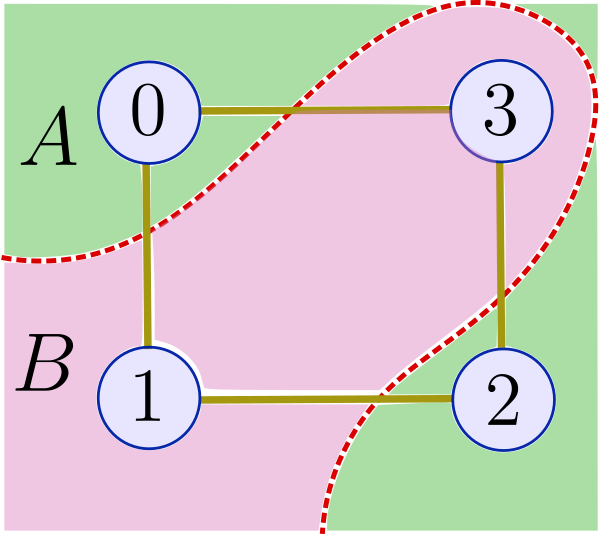
\includegraphics[scale = 0.8]{img/03-max_cut_problem.png}
    \caption{representación del problema Max Cut}
    Fuente: adaptada de \cite{pn}.
    \label{fig:max_cut_problem}
\end{figure}

\newpage

El problema Max Cut, admite una formulación \mbox{QUBO} natural dada por la expresión \ref{eq:max_cut_problem_max}.

\begin{equation}
    \text{Maximizar} \quad f(\Vec{x}) = \sum_{(i,j) \in E} (x_i + x_j -2x_ix_j)
    \label{eq:max_cut_problem_max}
\end{equation}

La expresión \ref{eq:max_cut_problem_max} modeliza el problema que se desea resolver, donde el valor de las variables binarias marca a que subconjunto pertenece cada uno de los vértices $V$ del grafo, siendo los de valor $0$ el primer subconjunto y los de valor $1$, los del segundo subconjunto. \\


Dado que se desea maximizar la expresión \ref{eq:max_cut_problem_max}, se necesita que para  el máximo número de aristas posible, el término $x_i + x_j -2 x_i x_j$  sea positivo no nulo y esto solo ocurre cuando las variables $x_i$ y $x_j$ toman valores diferentes. Para ello, necesariamente $x_i$ y $x_j$ deben pertenecer a subconjuntos distintos, ya que es la única combinación posible en la cual el termino del sumando es no nulo y positivo. \\

Tal y como está definido \ref{eq:max_cut_problem_max}, se trata de un problema de maximización, sin embargo si deseamos tratar el problema como un problema de minimización, podemos añadir un signo negativo global a la función, aprovechando la equivalencia de $max\{ f(x)\} = - \; min\{ - f(x) \}$. Esto transforma el problema Max Cut en un problema de minimización, tal y como viene dado en la expresión \ref{eq:max_cut_problem_min}, lo cual es mas adecuado para nuestros propósitos.

\begin{equation}
    \text{Minimizar} \quad f(\Vec{x}) = - \sum_{(i,j) \in E} (x_i + x_j - 2x_i x_j)
    \label{eq:max_cut_problem_min}
\end{equation}

La expresión objetivo se convierte ahora en una función cuyo mínimo, en valor absoluto, representa el valor solución del problema. El problema Max Cut, aunque simple, es un problema base que posee aplicaciones directas en ámbitos como la inteligencia artificial o el diseño de circuitos. El problema Max Cut tiene una representación dual, ya sea en forma de grafo o en forma de las expresiones \ref{eq:max_cut_problem_max} y \ref{eq:max_cut_problem_min}. Con el objetivo de generar un conjunto suficientemente grande de problemas Max Cut, se va a utilizar un generador de grafos de tipo Erdös–Rényi \citep{li}. Un grafo de tipo Erdös $G(n,p)$, es aquel grafo que posee $n$ vértices con una probabilidad de conexión con el resto de vértices de $p$. Este tipo de grafos permite, dado un tamaño y una probabilidad de conexión, generar un conjunto grande de problemas Max Cut. 

\newpage


\section{Algoritmos variacionales cuánticos}

En está sección se presentan la clase de algoritmos cuánticos utilizados en el desarrollo de trabajo. Los algoritmos cuánticos variacionales \citep{cerezo} conforma un subconjunto de algoritmos cuánticos orientados a la resolución de problemas de optimización. Uno de los conceptos centrales en este tipo de algoritmos cuánticos es el de Hamiltoniano, ya que estos algoritmos están orientados a encontrar cual es el estado de mínima energía del sistema, es decir, cual es el vector o vectores propios del Hamiltoniano de menor energía. \\


El Hamiltoniano no es un operador unitario, a diferencia de las puertas cuánticas, dado que el objetivo de este operador no es actuar sobre los qubits para cambiar su estado, si no conocer la energía del estado en el que se encuentra el sistema cuántico. Formalmente, la acción del Hamiltoniano, $H$ sobre un estado del sistema $\ket{\psi}$ viene dado por la ecuación \ref{eq:autovalor_h}.

\begin{equation}
    H \ket{\psi} = E \ket{\psi}
    \label{eq:autovalor_h}
\end{equation}

La ecuación \ref{eq:autovalor_h} se denomina ecuación de autovalores y permite obtener la energía de cada estado $\ket{\psi}$ del sistema. Este hecho permite mostrar una analogía entre la ecuación de autovalores con la evaluación de una función \mbox{QUBO} $f(\Vec{x})$, para un conjunto de valores dados de las variables binarias. Dado un vector $\ket{\psi}$ la ecuación \ref{eq:autovalor_h} nos devuelve el valor $E$ asociado para un $H$ especifico, del mismo modo que dado un vector de variables fijadas $\Vec{x}_{0}$, la evaluación $f(\Vec{x}_0)$ nos devuelve el valor de $f(\Vec{x})$ en el estado $\Vec{x}_0$. Se puede establecer una relación matematica entre las formulaciones \mbox{QUBO} clásicas de los problemas y formulaciones cuánticas mediante Hamiltonianos. Existe un mapeo directo de la formulación \mbox{QUBO} a una formulación cuántica mediante Hamiltonianos denominada formulación Ising. La transformación entre formulaciones \mbox{QUBO}-Ising viene dada por la expresión \ref{eq:qubo_ising}.

\begin{equation}
    x_{i} \longrightarrow \frac{1 - Z_{i}}{2}
    \label{eq:qubo_ising}
\end{equation}

Donde $Z_{i}$ representa el operador o puerta cuántica de Pauli $Z$ actuando sobre el qubit i-ésimo. Se pasa de un problema de variables binarias con valores $0$ y $1$ en formulación \mbox{QUBO}, a variables con valores $1$ y $-1$, en formulación Ising. Esta regla permite traducir de forma directa un problema \mbox{QUBO}, escrito en terminos de variables binarias clásicas, a un Ising, escrito en terminos de operadores cuánticos \citep{lucas}.

\newpage

En formulación Ising el problema Max Cut presentado en el apartado \ref{sub:problem_target} viene dada por la expresión \ref{eq:problem_ising_target}, en la versión de minimización.

\begin{equation}
    \text{Minimizar} \quad H =  - \frac{1}{2}\sum_{(i,j) \in E} (1 - Z_i Z_j)
    \label{eq:problem_ising_target}
\end{equation}

Podemos ahora introducir el funcionamiento de los algoritmos cuánticos variacionales una vez entendida la relación entre la formulación de Hamiltonianos y la formulación  \mbox{QUBO} de problemas clásicos. Los algoritmos variacionales cuánticos hacen uso del denominado principio variacional de Rayleigh-Ritz \citep{fernandez}. El principio viene expresado matemáticamente por la ecuación \ref{eq:variational_principle}.

\begin{equation}
    \bra{\psi} H \ket{\psi} \geq E_{0}
    \label{eq:variational_principle}
\end{equation}

El principio variacional determina que el valor esperado del Hamiltoniano, la energía del sistema que es observada, se minimiza cuando $\ket{\psi}$ representa el estado fundamental del sistema cuántico. Para cualquier otro estado genérico $\ket{\psi_{i}}$ el valor esperado, $E_{i}$, siempre es mayor que el valor mínimo $E_{0}$. Esto permite establecer un criterio de búsqueda para encontrar el estado $\ket{\psi}$ que representa el estado fundamental del sistema, ya que será este estado el que minimice la ecuación \ref{eq:variational_principle}. Los algoritmos variacionales cuánticos hacen uso de este principio para encontrar el estado $\ket{\psi}$ que minimiza el valor esperado del Hamiltoniano. En terminos clásicos esto es equivalente a encontrar el vector de parámetros $\Vec{x}$ que minimiza la función de coste $f(\Vec{x})$. \\

El primer algoritmo variacional cuántico propuesto, fue el denominado  Variational Quantum Eigensolver, o VQE \citep{peruzzo} por sus siglas en inglés. El flujo de trabajo del algoritmo VQE puede resumirse mediante la Figura \ref{fig:vqe}. El algoritmo VQE como algoritmo híbrido clásico-cuántico consta de dos partes bien diferenciadas. En un primer paso, el ordenador cuántico prepara un estado cuántico $\ket{\psi(\Vec{\theta})}$ que depende de un conjunto de parámetros $\Vec{\theta}$. Esto se consigue mediante los denominados \mbox{PQC} o circuitos cuánticos parametrizados, los cuales son una secuencia de puertas cuánticas que actúan sobre los qubits y que dependen de un conjunto de parámetros $\Vec{\theta}$.

\newpage

\begin{figure}[!ht]
    \centering
    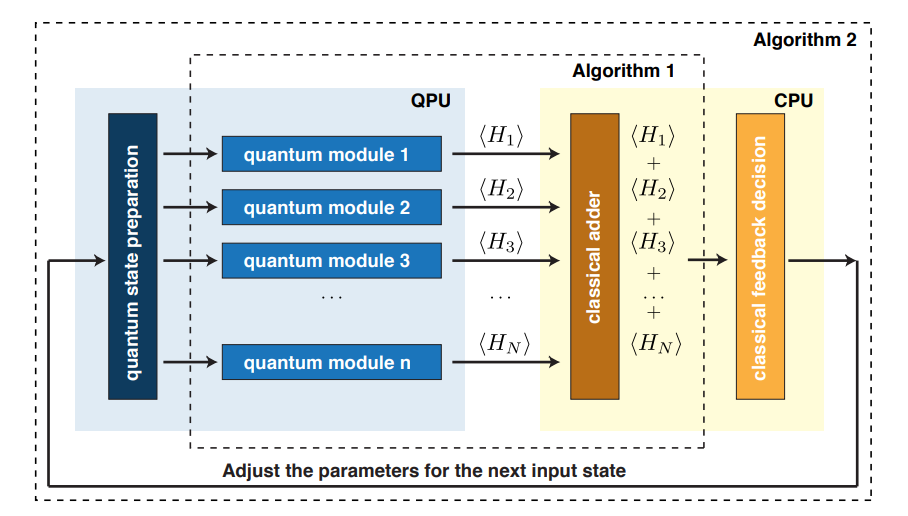
\includegraphics[scale = 0.7]{img/03-vqe_workflow.png}
    \caption{flujo de trabajo del algoritmo VQE.}
    Fuente: adaptada de \cite{peruzzo}.
    \label{fig:vqe}
\end{figure}

La construcción del estado $\ket{\psi(\Vec{\theta})}$ viene dado por la expresión \ref{eq:pqc}.

\begin{equation}
    |\psi(\boldsymbol{\Vec{\theta}}) \rangle = U(\boldsymbol{\Vec{\theta}}) |0\rangle^{\otimes n}
    \label{eq:pqc}
\end{equation}

Donde $U(\boldsymbol{\Vec{\theta}})$ es el operador unitario que representa la acción del circuito cuántico parametrizado sobre los \textit{n} qubits, que se encuentran todos ellos en el estado $\ket{0}$. La acción del \mbox{PQC} se realiza descomponiendo el operador global en términos de operadores o puertas cuánticas de 1 y 2 qubits, tal y como se ve en la expresión \ref{eq:pqc_descompuesto}.

\begin{equation}
    U(\boldsymbol{\Vec{\theta}}) = U_n(\theta_n) U_{n-1}(\theta_{n-1}) \cdots U_1(\theta_1)
    \label{eq:pqc_descompuesto}
\end{equation}

Una vez el ordenador cuántico ha preparado el sistema en el estado $\ket{\psi(\Vec{\theta})}$, el siguiente paso es el calculo del valor esperado del Hamiltoniano que codifica el problema que nos interesa resolver. Una vez calculado el valor esperado del Hamiltoniano, un ordenador clásico analiza el resultado y calcula un nuevo vector de parámetros $\Vec{\theta'}$ para construir un nuevo estado $\ket{\psi(\Vec{\theta'})}$. Este nuevo estado $\ket{\psi(\Vec{\theta'})}$ a su vez se utiliza para calcular el valor del Hamiltoniano para posteriormente actualizar los parámetros $\Vec{\theta}$ del circuito cuántico parametrizado.

\newpage

Realizando este proceso de forma iterativa, se llegará en un numero finito de pasos a un circuito cuántico parametrizado que genere un estado $\ket{\psi(\Vec{\theta_{final}})}$, el cual minimiza el valor esperado del Hamiltoniano. Por el principio variacional, este vector representa el estado que minimiza la energía del sistema, o lo que es lo mismo, el estado fundamental. Se ha encontrado así el estado que minimiza el Hamiltoniano o en terminos de formulación \mbox{QUBO}, se ha encontrado el valor de las variables binarias que minimiza la función de coste $f$. \\

Posterior a la aparición del algoritmo VQE, numerosos algoritmos cuánticos variacionales han surgido en la literatura académica. Uno de los mas destacados es el algoritmo Quantum Approximate Optimization Algorithm, o QAOA \citep{farhi} por sus siglas en inglés. La diferencia principal entre el algoritmo QAOA y el algoritmo VQE es el tipo de circuito cuántico parametrizado se usa para la preparación del estado  $\ket{\psi(\Vec{\theta})}$. En el algoritmo QAOA el circuito encargado de construir un estado parametrizado $\ket{\psi(\Vec{\theta})}$ viene dado por la expresión \ref{eq:pqc_qaoa}.


\begin{equation}
    U(\vec \gamma,\vec \beta)=\prod_{k=1}^p e^{-i \gamma_k H_C} e^{- i \beta_k H_M}
    \label{eq:pqc_qaoa}
\end{equation}

Donde $H_C$ hace referencia al Hamiltoniano problema y $H_M=-\sum_{i=1}^n X_i$, al denominado Hamiltoniano de mezcla. El productorio implica la aplicación de $p$ capas, de los operadores $e^{-i \gamma_k H_C}$ y $e^{- i \beta_k H_M}$, que actúan sobre el estado base. En la Figura \ref{fig:qaoa_layers} se puede observar la estructura de $p$ capas para construir un estado parametrizado.

\begin{figure}[!ht]
    \centering
    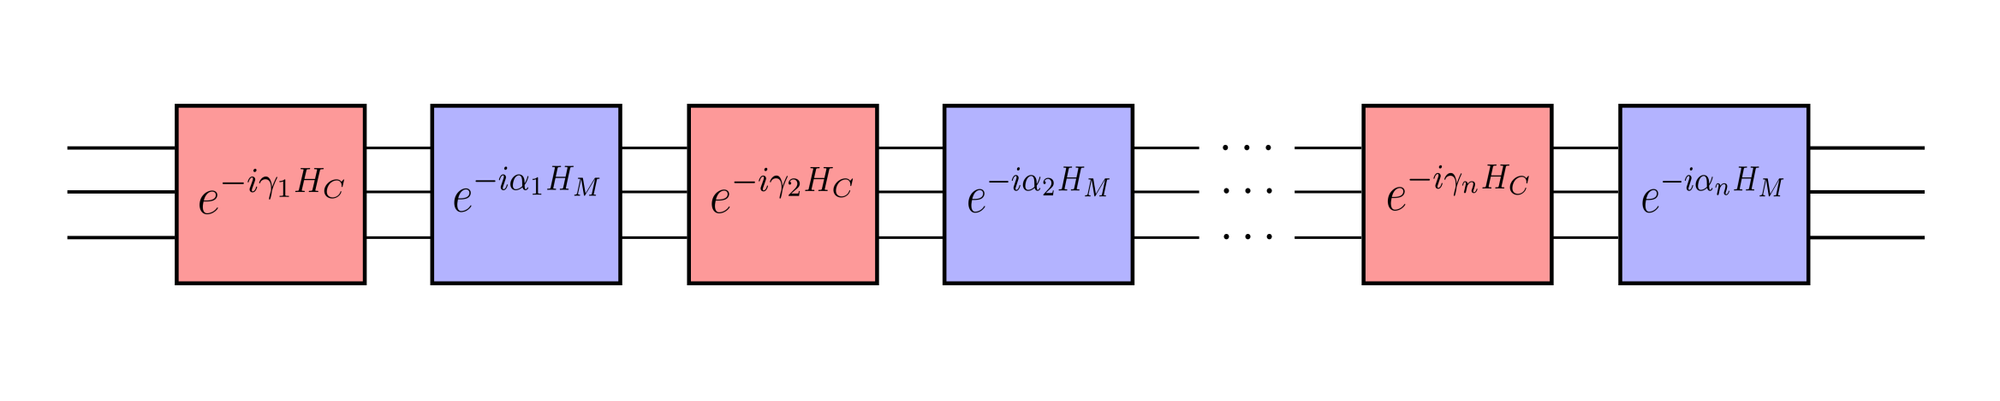
\includegraphics[scale = 0.4]{img/03-qaoa_layers.png}
    \caption{esquema de \mbox{PQC} para el algoritmo QAOA.}
    Fuente: adaptada de \cite{jack}
    \label{fig:qaoa_layers}
\end{figure}

Los operadores expresados como exponenciales complejas pueden implementarse a través de una secuencia de puertas cuánticas de 1 y 2 qubits. El resto del funcionamiento de algoritmo es equivalente al del algoritmo VQE. 

\newpage

Una vez construido el estado parametrizado, $\ket{\psi(\Vec{\gamma}, \Vec{\beta})}$, se evalúa el valor esperado del Hamiltoniano para posteriormente, gracias a un ordenador clásico que implementa un optimizador, se actualizan el conjunto de parámetros para reducir el valor esperado de la energía del sistema. En general cualquier algoritmo cuántico variacional consta de tres componentes principalmente. 

\begin{itemize}
    
    \item Circuito cuántico parametrizado o \mbox{PQC}: conjunto y estructura de puertas cuánticas utilizadas para preparar el estado inicial en un ordenador cuántico. Contiene los parámetros variacionales que pueden ajustarse durante el proceso de optimización.

    \item Optimizador clásico: el optimizador clásico se encarga de ajustar los parámetros variacionales en el \mbox{PQC} para minimizar la función de coste. Utiliza técnicas clásicas de optimización para encontrar el conjunto óptimo de parámetros que produzcan el resultado deseado.

    \item Función de coste: la función de coste cuantifica el objetivo que el algoritmo variacional pretende optimizar. Evalúa la calidad de la salida obtenida del circuito cuántico. El objetivo es minimizar la función de coste ajustando los parámetros variacionales.
    
\end{itemize}

Puede afirmarse que tanto el algoritmo VQE como el algoritmo QAOA son los algoritmos fundacionales dentro de los algoritmos cuánticos variacionales. Numerosos algoritmos han surgido como versiones modificadas y mejoradas tanto del algoritmo VQE como del algoritmo QAOA. Por ejemplo, el algoritmo F-VQE \citep{amaro} implementa un optimizador clásico nativo basado en el descenso del gradiente. Otras versiones modificadas del algoritmo VQE como el algoritmo MOVCO \citep{luis}, implementan dos funciones de coste que deben ser optimizadas de forma simultánea. Así mismo, también se han desarrollado numerosas versiones del algoritmo QAOA, como el ADAPT-QAOA \citep{zhu}, en el cual cada una de las capas del QAOA se optimiza de forma iterativa y dónde el circuito cuántico parametrizado se construye de forma dinámica. \\

El objetivo de todas las versiones surgidas posteriores a los algoritmos VQE y QAOA originales tratan de mitigar y superar las deficiencias que existen en esta clase de algoritmos. Los problemas que presentan esta clase de algoritmos están asociados principalmente a que no aseguran la convergencia a soluciones que sean óptimos globales.

\newpage

Otro problema asociado se debe al efecto de \textit{Barren Plateaus} \citep{mcClean}, un fenómeno por el cual las superficies de energía, de las funciones de costo, exhiben zonas casi planas en el paisaje de la función objetivo. Esto significa que los gradientes de la función (es decir, las direcciones en las que cambia más rápidamente la función) se vuelven extremadamente pequeños o cercanos a cero en muchas partes del espacio de parámetros. La presencia de estas \textit{Barren Plateaus} puede ser problemática para los algoritmos de optimización cuántica, ya que los métodos estándar que confían en la exploración guiada por gradientes pueden volverse ineficaces. 

\section{Introducción a tensor networks}


Tensor networks \citep{orus} es una técnica y herramienta fundamental en física teórica y materia condensada que permite representar estados cuánticos complejos y realizar cálculos eficientes en sistemas de muchas partículas. En una tensor network, un estado cuántico se descompone en un conjunto de tensores interconectados, donde cada tensor representa una parte localizada del sistema. La estructura y disposición de estos tensores captura las correlaciones cuánticas entre las distintas partes del sistema. \\

La utilidad de las tensor networks radica en su capacidad para manejar estados cuánticos de alta dimensionalidad de manera eficiente. Por ejemplo, en sistemas cuánticos con muchas partículas, representar directamente el estado completo sería computacionalmente prohibitivo debido a la explosión combinatoria de las dimensiones. Sin embargo, mediante una representación basada en tensor networks, podemos enfocarnos en las correlaciones locales significativas y omitir aquellas que son menos relevantes, reduciendo así el coste computacional. Es decir, permite un manejo eficiente de sistemas cuánticos grades que bajo otro formalismo no sería factible. \\


Las tensor networks se han aplicado con éxito en diversas áreas, incluida la simulación de materia condensada y sistemas cuánticos, donde permiten estudiar propiedades como la energía, la magnetización y las funciones de correlación. Además, han encontrado aplicaciones en el campo emergente del aprendizaje automático \citep{chen}. 

\newpage

Dado un estado cuántico $\ket{\psi}$, se puede expresar dicho estado cuántico en términos de una combinación lineal de los estados base, que para el caso particular de un solo qubit, son los estados $\ket{0}$ y $\ket{1}$. La expansión genérica de un estado de $N$ qubits viene dado por la expresión \ref{eq:psi_expansion}.

\begin{equation}
    \ket{\psi} = \sum_{i_1, i_2, ...,i_N} C_{i_1, i_2, ...,i_N} \ket{i_1}\otimes\ket{i_2}\otimes...\otimes \ket{i_N}
    \label{eq:psi_expansion}
\end{equation}

Donde los estados $\ket{i_1}\otimes\ket{i_2}\otimes...\otimes \ket{i_N}$ son los estados de la base del estado $\ket{\psi}$ expresado en términos de los estados base $\ket{i_s}$ de cada uno de los qubits del sistema. Los coeficientes $C_{i_1, i_2, ...,i_N}$ de la expansión puede entenderse como un tensor que posee $N$ índices, cada uno de los cuales puede tomar valores distintos. Gráficamente puede representarse en el formalismo de tensor networks al tensor $C$ tal y como se observa en la Figura \ref{fig:orus}.

\begin{figure}[!ht]
    \centering
    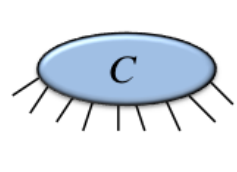
\includegraphics[scale = 0.8]{img/03_tensor_coeficientes.png}
    \caption{representación del tensor de coeficientes $C$  de la expansión del estado $\ket{\psi}$.}
    Fuente: adaptada de \cite{orus}
    \label{fig:orus}
\end{figure}

En la Figura \ref{fig:orus} cada una de las patas del tensor $C$ representa cada uno de los índices del tensor. Sin embargo, la dimesionalidad del tensor $C$ es enorme para sistemas cuánticos de muchos qubits o partículas, por lo que es necesario descomponer el tensor $C$ en terminos de tensores mas pequeños para poder trabajar de forma eficiente con el. Formalmente y siguiendo la regla de índices de Einstein \citep{ahlander}, un tensor $C$ puede expresarse como producto de varios tensores de menor rango, menor dimesionalidad, tal y como se muestra en la expresión \ref{eq:contracction}.

\begin{equation}
    C_{i j} = \sum_{\alpha} A_{i  \alpha} B_{\alpha j} = A_{i  \alpha} B^{\alpha j}
    \label{eq:contracction}
\end{equation}

Esto permite expresar un tensor arbitrariamente grande en terminos de una descomposición de tensores de menor dimensión. Graficamente, esta descomposición puede dar lugar a distintas redes de tensores, dado que la descomposición de un tensor no es única. En la Figura \ref{fig:c_descomposition} pueden observarse distintas posibles descomposiciones del tensor $C$ en terminos de tensores de menor dimesionalidad.


\begin{figure}[!ht]
    \centering
    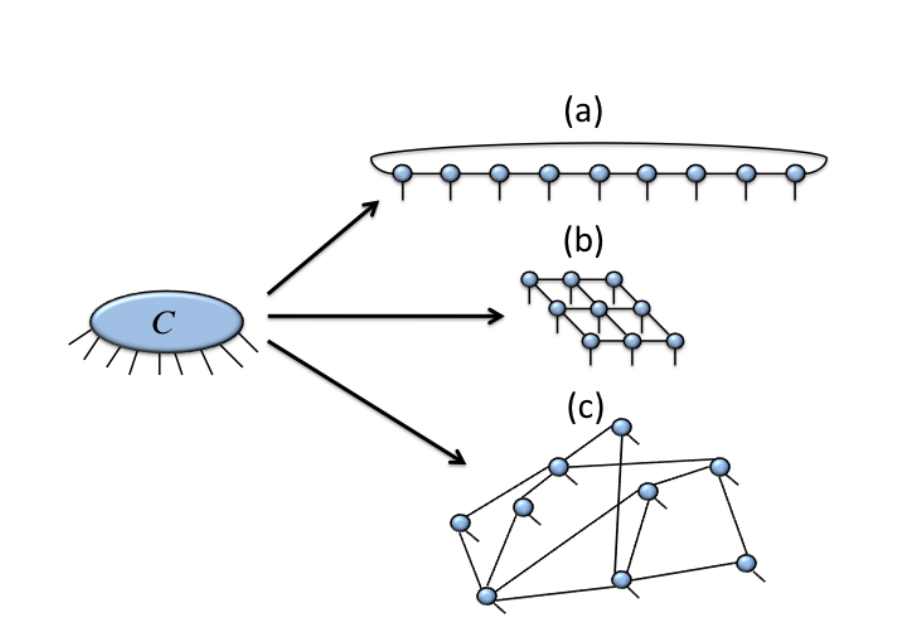
\includegraphics[scale = 0.7]{img/03-tensor_descomposicion.png}
    \caption{descomposición del tensor $C$ en distintas redes tensoriales.}
    Fuente: adaptada de \cite{orus} 
    \label{fig:c_descomposition}
\end{figure}

\newpage

Las patas internas, aristas que unen entre sí a los tensores, de la red tensorial representan los índices de los tensores que se contraen, tal y como dicta la ecuación \ref{eq:contracction} para poder obtener el tensor $C$. Por otro lado, las patas abiertas, representan los índices físicos del tensor $C$, las patas originales del tensor que no aparecen por la descomposición, ya que al contraer la red, estos índices sobreviven. La figura $(a)$ de la imagen \ref{fig:c_descomposition} representa un tipo especifico de descomposición denominada Matrix Product State, o MPS por sus siglas en inglés, y es una representación especialmente conveniente para simular sistemas en computación cuántica. Bajo la representación MPS, cada tensor de la red corresponde con un qubit del sistema cuántico, donde cada índice o pata abierta corresponde con la dimensión física del qubit. En el trabajo desarrollado en este documento se hará uso de la representación MPS para realizar simulaciones eficientes de sistemas cuánticos. Es importante tener en cuenta, que bajo este formalismo podemos realizar simulaciones eficientes de sistemas cuánticos, pero simulaciones no exactas. El parámetro que dicta que tan buena es la aproximación entre la simulación aproximada y la exacta es la dimensión $D$ de los índices internos de la red de tensores. Cuanto mayor sea el valor de $D$ mejor será la aproximación. La dimensión de los índices internos determinan la cantidad de correlaciones que la red de tensores es capaz de capturar del sistema cuántico. Un sistema cuántico con correlaciones entre los qubits baja, requiere un valor bajo de $D$ para poder ser simulado de forma suficientemente buena. En la Figura \ref{fig:mps_hilbert_space} podemos ver como la dimensión interna de los índices de la red impacta en el tamaño del espacio de Hilbert total que es capaz de capturar en la representación MPS.


\begin{figure}[!ht]
\centering
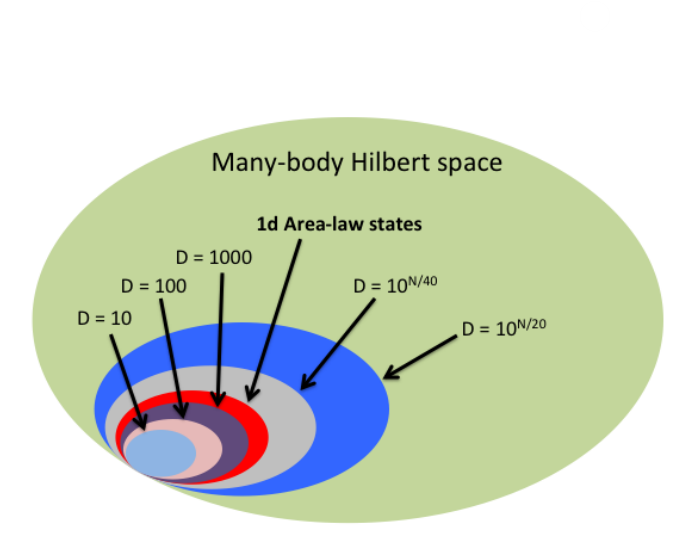
\includegraphics[scale = 0.55]{img/03-mps_espacio_hilbert.png}
\caption{subespacio de Hilbert que es capaz de representar una red MPS en función de la dimensión interna $D$ para un sistema de $N$ qubits.}
Fuente: adaptada de \cite{orus} 
\label{fig:mps_hilbert_space}
\end{figure}

Sin embargo, aumentar la dimensión interna de la red de tensores conlleva un coste computacional, ya que por la ecuación \ref{eq:contracction}, el aumento de la dimensión implica un aumento en el numero de productos y sumas a realizar cuando se quieren contraer dos tensores de la red. Es necesario fijar una dimensión interna suficientemente alta para realizar simulaciones fidedignas pero que no impliquen un coste computacional prohibitivo. De esta forma podemos realizar simulaciones eficientes de estados cuánticos. \\

Bajo el formalismo de tensor networks, las puertas cuánticas de un qubit se entienden como matrices, tensores de dos índices, las cuales pueden operar sobre estados cuánticos en forma de MPS simplemente contrayendo el índice de entrada de la puerta cuántica sobre el índice físico del tensor, qubit, correspondientes del estado MPS. Para el caso de puertas de dos qubits, tenemos tensores de cuatro índices, dos de entrada y dos de salida. \\

\newpage

Además de entender como representar estados cuánticos de forma eficiente bajo el formalismo de tensor networks, es necesario entender también como codificar Hamiltonianos en este paradigma. Existe un objeto en tensor networks el cual es una extensión natural de los estados MPS, denominados Matrix Product Operator o MPO, por sus siglas en inglés. Un operador MPO es una tensor network donde cada tensor tiene dos patas no contraídas, así como dos patas internas que conectan con los tensores vecinos en forma de cadena, tal y como puede visualizarse en la Figura \ref{fig:mpo}.


\begin{figure}[!ht]
    \centering
    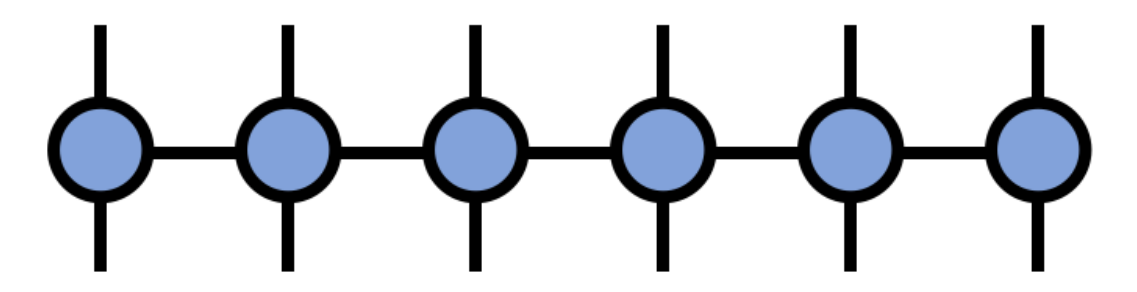
\includegraphics[scale = 0.35]{img/03-mpo.png}
    \caption{representación de un MPO}
    Fuente: adaptada de \cite{tn} 
    \label{fig:mpo}
\end{figure}

De igual manera que un estado MPS representa un estado cuántico, el MPO representa un operador cuántico. Existen diversas formas de construir el MPO a partir de un Hamiltoniano. Para Hamiltonianos con interacciones no locales, es decir Hamiltonianos donde los qubits interactúan entre sí, independientemente de si son vecinos o no, la construcción del operador MPO no es trivial. Se han propuesto reglas \citep{fröwis} para poder construir de forma eficiente MPO's que representen Hamiltonianos genéricos que contengan interacciones no locales. De forma general un operador se puede describir a través de la expresión \ref{eq:operator}.

\begin{equation}
    H = \sum_{i} \sum_{i'} C_{i_1 i_2 \ldots i_L}^{i'_1 i'_2 \ldots i'_L} \left| i_1 i_2 \ldots i_L \right\rangle \left\langle i'_1 i'_2 \ldots i'_L \right|
    \label{eq:operator}
\end{equation}

De forma análoga a lo realizado para los estados $\ket{\psi}$, podemos descomponer el tensor $ C_{i_1 i_2 \ldots i_L}^{i'_1 i'_2 \ldots i'_L}$ en tensores de menor dimensión. Esta descomposición del tensor, que representa en el operador Hamiltoniano, en tensores de menor dimensión es lo que da lugar a la representación en forma de MPO de un operador tal y como hemos visto en la figura \ref{fig:mpo}. \\


Bajo el paradigma de tensor networks, la ecuación \ref{eq:autovalor_h} viene dada por la contracción del estado $\ket{\psi}$ sobre el MPO que representa el operador $H$. En la Figura \ref{fig:mpo_to_mps} se observa en forma tensorial la ecuación de autovalores dada por la acción del MPS sobre el MPO.

\newpage

\begin{figure}[!ht]
    \centering
    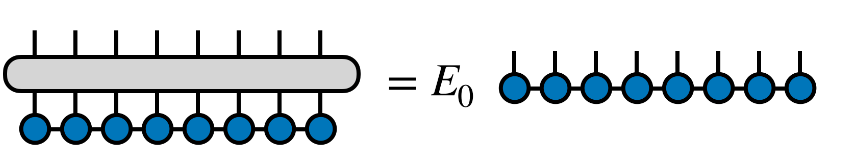
\includegraphics[scale = 0.65]{img/03-mpo_to_mps.png}
    \caption{representación en forma tensorial de la ecuación de autovalores}
    Fuente: adaptada de \cite{tn} 
    \label{fig:mpo_to_mps}
\end{figure}

Los conceptos de MPS y MPO para la representación de estados cuánticos y operadores, respectivamente, son las ideas más importantes, dentro del campo de las tensor networks, para el desarrollo del trabajo realizado. 


\section{Computación cuántica en entornos industriales}

Es necesario contextualizar el estado teórico de los algoritmos cuánticos, de los cuales se pretenden hacer uso, con el estado del hardware en los cuales deben ejecutarse. Actualmente nos encontramos en la época denominada de ordenadores ruidosos de escala intermedia \citep{preskill} o NISQ por sus siglas en inglés. Las computadoras cuánticas en la era NISQ están limitadas en términos de la cantidad de qubits que poseen y la calidad de las operaciones cuánticas que pueden implementar. Esto significa que estas máquinas no están completamente libres de errores y tienen una capacidad de cómputo limitada en comparación con lo que se espera en sistemas cuánticos futuros. Los qubits en las máquinas NISQ son susceptibles a errores debido al ruido y la decoherencia cuántica. Estos errores pueden surgir debido a fluctuaciones ambientales y limitaciones tecnológicas en el control de los sistemas cuánticos. \\

La decoherencia es el fenómeno físico por el cual un estado cuántico $\ket{\psi}$ se destruye después de un tiempo dado, es decir, el tiempo de coherencia es la cantidad de tiempo que un estado cuántico $\ket{\psi}$ permanece, es decir, el tiempo en el que el sistema cuántico conserva la información. Actualmente el tiempo de coherencia de los ordenadores cuánticos impone una restricción fuerte en términos de la profundidad de los circuitos cuánticos que pueden ejecutarse. Dado que la profundidad del circuito no puede superar el tiempo de coherencia, esto provoca que los circuitos deban ser poco profundos y la cantidad de puertas cuánticas que se apliquen sean limitadas. Esto limita a su vez los algoritmos cuánticos que puede ser ejecutados actualmente en ordenadores cuánticos, siendo los algoritmos cuánticos variacionales de los pocos tipos de algoritmos que actualmente pueden ejecutarse de forma relativamente fiable en las plataformas cuánticas \citep{bharti}. \\

Otro problema asociado al estado actual del hardware se debe al costo económico por el acceso y uso de plataformas cuánticas reales. El número de ordenadores cuánticos disponibles es limitado. Esto supone que el acceso al uso y ejecución de estos ordenadores conlleva un gran costo económico asociado, por lo que utilizar algoritmos cuánticos para la resolución de problemas que requieran de un uso intensivo de ordenadores cuánticos puede ser inviable en términos de coste económico. 





